%%%%%%%%%%%%%%%%%%%%%%%%%%%%%%%%%%%%%%%%%%%%%%%%%%%%%%%%%%%%
%%%   Tracking and Analyzing The 2013 Italian Election   %%%
%%%%%%%%%%%%%%%%%%%%%%%%%%%%%%%%%%%%%%%%%%%%%%%%%%%%%%%%%%%%

\documentclass{llncs}

\newcommand{\superscript}[1]{\ensuremath{^{\textrm{#1}}}}

\usepackage{makeidx}  % allows for indexgeneration
\usepackage[hyphens]{url}
\usepackage{textcomp}
\usepackage{color}
\usepackage{listings}
\usepackage{multirow}
\usepackage{mathtools}
\usepackage{graphicx}
\usepackage{fancyvrb}
\usepackage{amsmath}
\usepackage{graphicx}
\usepackage[font=small,labelfont=bf]{caption}
\setcounter{MaxMatrixCols}{20}
\usepackage{pbox}
\usepackage{amsfonts}


% listing styles
\lstset{numbers=left, numberstyle=\tiny,basicstyle=\ttfamily\scriptsize, tabsize=2, keywordstyle=\underbar, stringstyle=\small, backgroundcolor=\color[gray]{0.94}, framexleftmargin=2pt}
\lstdefinestyle{rdfa}{numberblanklines=true, morekeywords={}}



\begin{document}
\frontmatter          % for the preliminaries
\pagestyle{headings}  % switches on printing of running heads
\mainmatter              % start of the contributions
\title{LinkedTV News \\ The 2013 Italian Election}
\titlerunning{Tracking and Analyzing The 2013 Italian Election}  % abbreviated title (for running head)

\title{LinkedTV News a companion application for newscasts}
\author{Michiel Hildebrand\inst{1}, Lilia Perez Romero\inst{1}, Jos\'e Luis Redondo Garc\'ia\inst{2}, Rapha\"el Troncy\inst{2}}
\institute{CWI, Amsterdam, The Netherlands, \\
\email{\{M.Hildebrand, L.Perez\}@cwi.nl}
\and
EURECOM, Sophia Antipolis, France, \\
\email{\{redondo, raphael.troncy\}@eurecom.fr}
}


\maketitle              % typeset the title of the contribution

%%%%%%%%%%%%%%%%%%
%%%  Abstract  %%%
%%%%%%%%%%%%%%%%%%

\begin{abstract}
The presence of appropriate TV content annotations and usage of custom visualization strategies are key factors to enhance the viewer experience. In this paper, we present an approach that leverages on the knowledge present on the Web for identifying and enriching relevant items inside a News video and displaying them in a timely and user friendly fashion. 
In particular, this second screen prototype (i) collects and offers information about persons, locations, organizations and concepts occurring in the newscast, and (ii) combines them for enriching the underlying story along five main dimensions: in other sources, expert's opinions, timeline of the news, in depth information, and geo-localized comments and remarks from other viewers.  
Starting from preliminary insights coming from the named entities spotted on the video subtitles, we expand this initial context to a broader event representation by relying in the knowledge of other non-structured Web documents talking about the same fact. This makes possible to generate a much richer, context aware metadata of a TV program that boost the viewer interaction and opens new possibilities in the hyperlinked television domain. 

\keywords{Television, Visual Summarization, Topic Generation}
\end{abstract}

%%%%%%%%%%%%%%%%%%%%%%%%%
%%%  1. Introduction  %%%
%%%%%%%%%%%%%%%%%%%%%%%%%

\section{Introduction}

People consume news from multiple sources, such as television, Web, radio and newspaper. Typically the activities using these sources are independent~\cite{}. For example, we watch the newscast on TV at a fixed time of the day to get an overview of the main news. We use the Web to keep track of the News throughout the day, and when we have more time to spare we actively browse the Web to explore the news items that we are interested in. At one hand this separation is natural as the activities have different characteristics and are integrated into our lifes in our way. At the other hand the different sources can complement each other and when consumed as such will enrich our news experience. The problem is that in practice it is difficult to manually link the different activities together. How often did you think of something you wanted to lookup on the Web while watching a newscast, but didn't, or while browsing the Web could not remember that one news item you saw on TV and wanted to explore further? 

% Semantic
The annotation problem has been traditionally addressed by applying multimedia analysis techniques \cite{ballan2011event}, but extracting semantic information from a video is still a challenging task. One possible approach consist in using Named Entity Recognition (NER) over the textual information attached to particular video fragment. Those techniques are an essential component within the Information Extraction field that focus on: identifying atomic information units in texts, named entities; classifying entities into predefined categories (also called context types) and linking to real world objects using web identifiers (Named Entity Disambiguation). A growing number of APIs provide such a service, like AlchemyAPI\footnote{\fontsize{8pt}{1em}\selectfont \url{http://www.alchemyapi.com/}} or DBpedia Spotlight\footnote{\fontsize{8pt}{1em}\selectfont \url{http://spotlight.dbpedia.org/}}. If the textual information attached to a video contains temporal references (e.g. subtitles), it is possible to align the entities with the time when they appear in the video. Katsiouli et al.~\cite{katsiouli2007} have demonstrated that applying named entity recognition techniques in combination with domain ontologies on video subtitles can produce good results for video classification.

%News Prototypes
Another example of content augmentation of news broadcasts is the work of Dowman et al. [3] Their system identifies individual stories in news broadcasts and annotates them with content from the World Wide Web. Annotations are used to produce summarized texts that can be employed potentially for enrichment of electronic programme guides. The focus of Dowman�s study is the technology that enables annotation. It presents an interface aimed for the postproduction (curating and editing) phase of the enriched hypermedia. This work relates to LinkedTV News in its integration of television newscasts with Web content. However it differs in that LinkedTV News is concerned with news consumption and not news postproduction.
Ardissono et al. [4] investigated personalization in the context of interactive news broadcasts through tracking and
inferring user content interests and media preferences. The authors describe the design and implementation of a broadcast news generator. This system combines automated video understanding and extraction together with user modeling to provide individualized personalcasts. We coincide with this work in that personalization should be an important ingredient in any an end-user hyperlinked news interface.

% SecondScreen
The employment of secondary devices for control of TV content was also explored in [12], where four major usages of the secondary screen in interactive television are identified and discussed: control, enrich, share and transfer television content.
Second screen multitasking is a growing practice that has triggered the interest of industry and stimulated the proliferation of commercial applications for dual device set- ups. One of the best known examples is Yahoo�s IntoNow [15]. IntoNow uses audio fingerprinting technology to automatically detect the program that users are watching and deliver related contents. 



%%%%%%%%%%%%%%%%%%
%%%  TV News  %%%
%%%%%%%%%%%%%%%%%%

\section{TV News}
\label{sec:tvnews}

LinkedTV News is a second screen application for tablets that acts as a companion to viewers when watching the news broadcasts.. Its main goal is to enrich television newscasts by integrating them with other media thus, integrating and concentrating the different activities related to getting informed about the news in one interactive multiple screen, and potentially mobile experience. It is designed to accommodate two viewing modes in terms of interaction: a lean back mode and a lean forward mode. 

In the passive mode the application operates as a second screen that is synced with the TV program. This mode supports the user with looking up factual information by presenting timed slides about the entities that occur in the news. As this mode requiers no interaction it unobtrusevely complements the lean back TV viewing experience. In addition, the passive mode provides functionality to bookmark news items. This one click interaction forms the bridge to the active mode of the application. 

In the active mode the user actively explores a specific news item. In this mode the application contains articles from the Web that are related to the news item in different dimensions. The dimension, such as articles from different news sources, opionion articles and a timeline of past events, are intended to support the specific user information needs that were identified in the study. While it is possible to use the active mode during the broadcast, this will disrupt the passive TV viewing experience. By first bookmarking the news item the user can come back to the application at a more appropriate time to start or continue the exploration.


\section{The lean back mode}
\label{sec:leanbackmode}

In this mode, the application presents the user with summarized additional information about elements of the news, for example, basic information about the location or people involved. This happens in the form of a slideshow with short texts and images that acts as a sort of news ticker to the broadcast appearing in the main screen. It automatically synchronizes with the TV, and requires no action from the user, but allows the user to browse slides, save them or bookmark news for later exploration. This lean back mode of the application intends to be as close as possible to a free hand, and passive experience. The slides are presented without need for user interaction, so the user can relax, share with her company and pay attention only to that which really calls her interest while easily bookmarking her favorite news for later reading. This favors an asynchronous mode of interaction that respects a passive mode of TV watching, and allows postponing the more attention demanding activities by using the TV program as an index for deciding what to explore in a more suitable time.


To reconstruct the semantic context associated with one particular news video, we extract the main concepts and entities from the subtitles and explain how they are related to each other. The complete processing workflow takes as input the textual transcript of a multimedia resource illustrating an event, as well as the start and end date for which that particular event is considered. We assume that this event has a minimal presence and coverage on the Web to ensure that the subsequent data mining techniques can collect sufficient data to reconstruct the event's context. 

For each news item, we perform named-entity recognition over the corresponding subtitles using the NERD framework~\cite{Rizzo2012b}. In our experiment, the language of the videos is English but NERD supports other languages. The output of this phase is a collection of entities annotated using the NERD Ontology\footnote{\fontsize{8pt}{1em}\selectfont \url{http://nerd.eurecom.fr/ontology/nerd-v0.5.n3}}, that comes with a first relevance score obtained from the extractors which have been used. This set includes a list of ranked entities that are explicitly mentioned during the video. Other entity based video annotation tools~\cite{yunjia2013} stop at this point even when entities that can be relevant for the viewer in the context of the event are still missing. We tackle this problem by extending this first list of concepts via the entity expansion component.

The set of entities obtained from a traditional named entity extraction operation is normally insufficient and incomplete for expressing the context of a news event. Sometimes, some entities spotted over a particular document are not disambiguated because the textual clues surrounding the entity are not precise enough for the name entity extractor, while in other cases, they are simply not mentioned in the transcripts while being relevant for understanding the story. We perform the a process named entity expansion operation, which relies on the idea of retrieving and analyzing additional documents from the Web where the same event is also described. By increasing the size of set of documents to analyse, we increase the completeness of the context and the representativeness of the list of entities, reinforcing relevant entities and finding new ones that are potentially interesting inside the context of that news item.

The entire logic is illustrated in in Figure~\ref{fig:namedEntityExpansion} and consists mainly in (1) building an appropriate search query from the original set of entities, (2) retrieving additional documents about the same news event, and (3) analyzing them for providing a more complete and better ranked set of final entities, as illustrated in Figure~\ref{fig:namedEntityExpansion}.

\begin{figure}[h!]
\centering
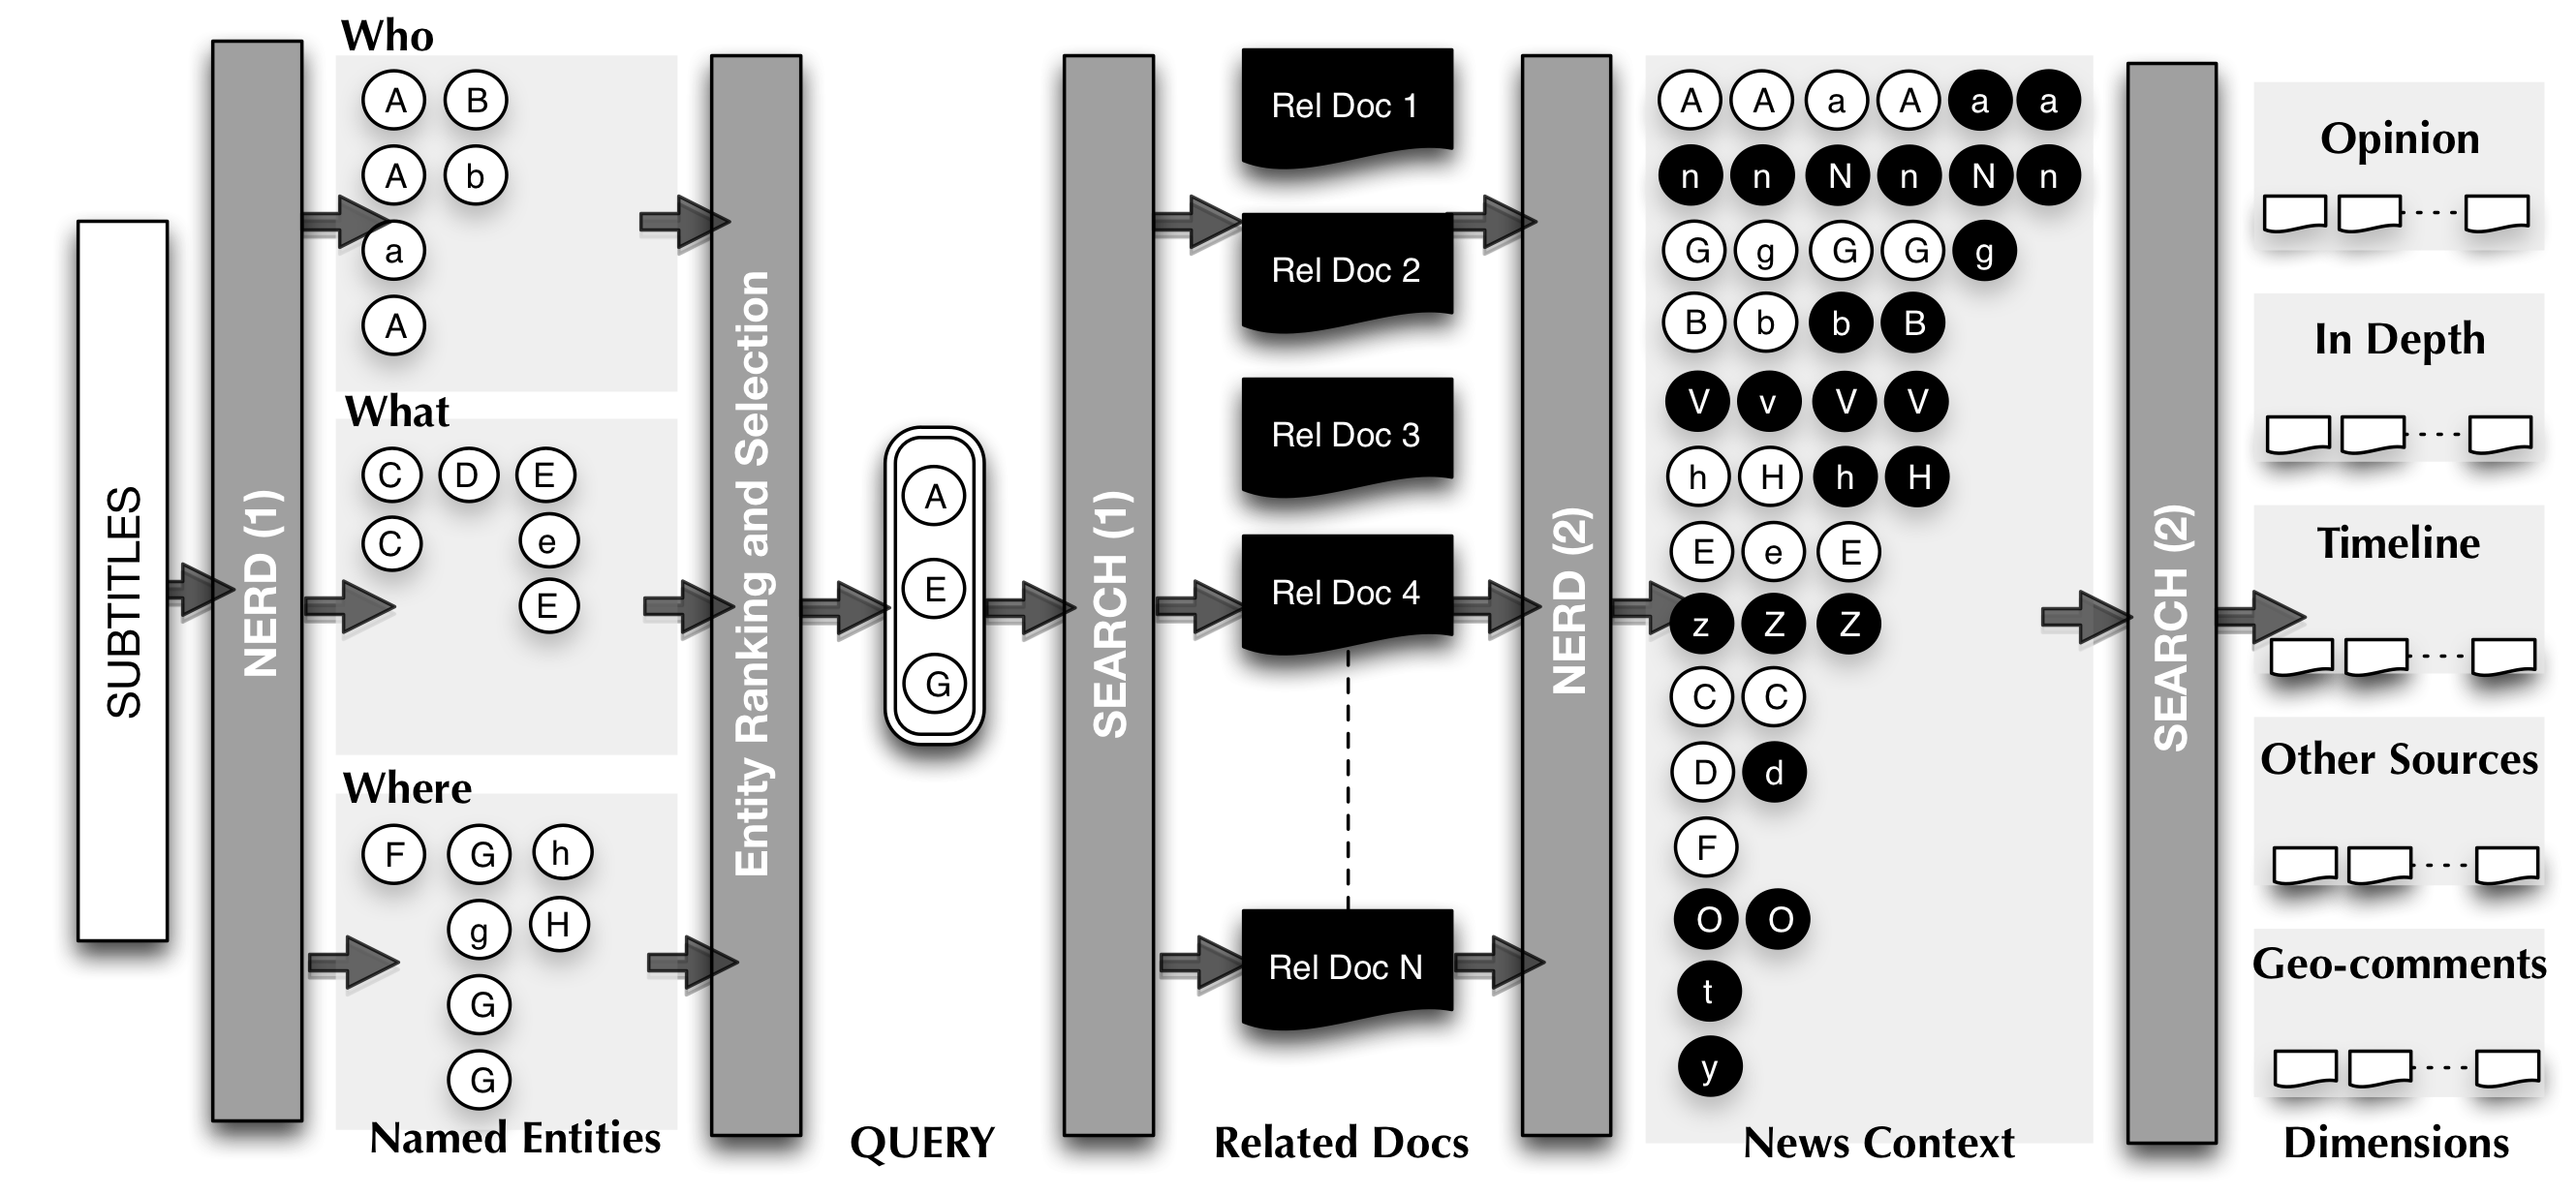
\includegraphics[width=0.6\textwidth]{figure/ExpansionDiagram}
\caption{Schema of Named Entity Expansion Algorithm.}
\label{fig:namedEntityExpansion}%\end{figure}
\end{figure}

The \emph{Five W's} is a popular concept of information gathering in journalistic reporting. It captures the main aspects of a story: who, when, what, where, and why~\cite{LiJia2007}. We try to represent the news item in terms of four of those five W's (who is involved in the event, where the event is taking place, what the event is about, and when it has happened) in order to generate a query that retrieves documents associated to the same event.

First, the original entities are mapped to the NERD Core ontology, which considers 10 main classes: Thing, Amount, Animal, Event, Function, Organization, Location, Person, Product and Time. From those ten different categories, we generalize to three classes: the Who from \url{nerd:Person} and \url{nerd:Organization}, the Where from \url{nerd:Location}, and the What from the rest of NERD types after discarding \url{nerd:Time} and \url{nerd:Amount}. The When or so-called temporal dimension does not need to be computed since it is considered to be provided by the video publisher.

After generating the three sets of entities, the next step consist in ranking them in relevance according to a weighted sum of two different dimensions: their frequency in the transcripts and their former relevance scores coming from the named entity extractors. We have defined the function \emph{filterEntities(S)} for selecting the $n$ entities inside the set of entities $S$ whose relative relevance falls into the upper quarter of the interval.

The final query is a pair where \textit{textQuery} is the result of concatenating the labels of the most relevant entities in the sets Who, What, Where in that particular order, and $t$ the time period dimension. This query generation is depicted in the upper part of Figure~\ref{fig:namedEntityExpansion}.

\subsubsection{Document Retrieval}
Once $\text{Query}_{Event}$ is built out of the original set of named entities, it will be ready to be injected into a document search engine where additional descriptions about the news event can be found. In this situation, the kind of query generated in the previous step and the search engine chosen should be closely tied in order to maximize the quality of the obtained results. The different behavior of search engines make some alternatives more suitable than others for certain kinds of events. The way the resulting documents change in the search engines for a particular kind of event is a research question that will not be studied in this paper.

In this paper, we rely on the Google Search REST API service\footnote{\fontsize{8pt}{1em}\selectfont  \url{http://ajax.googleapis.com/ajax/services/search/web?v=1.0}} by launching a query with the text \textit{textQuery}. Due to quota restrictions imposed by Google, the maximum number of retrieved document is set to 30. However, as shown in the evaluation described in the Section~\ref{sec:evaluation}, this is enough for significantly extending the initial set of entities directly spotted by NERD.

Concerning the temporal dimension, we only keep the documents published in the time period $t+t_{e}$. We increase the original event period in $t_{e}$ because documents concerning a news event are not always published during the time of the action is taking place but some hours or days after. The value of $t_{e}$ depends on many factors such as the nature of the event itself (whether it is a brief appearance in a media, or part of a longer story with more repercussion) or the kind of documents the search engine is indexing (from very deep and elaborated documents that need time to be published, to short post quickly generated by users). Based on the simple assumption that that the longer is an event, and the longer it is likely to generate buzzes, we approximated  $t_{e} = t$ which means that we also consider document published during the course of an event.

The middle part of Figure~\ref{fig:namedEntityExpansion} shows this process. The query is input in the search engine in order to retrieve other documents that report on the same event discussed in the original video. Those documents (colored in black in the Figure~\ref{fig:namedEntityExpansion}) will be further processed to increase the size of the collection and get additional insights about the news item.

\subsubsection{Entity Clustering}
In this phase, the additional documents which have just been retrieved are now processed and analyzed in order to extend and re-rank the original set of entities and consequently get a better insight about the event. Since most of the resources retrieved are Web pages, HTML tags and other annotations are removed, keeping only the main textual information. This plain text is then analyzed by the NERD framework in order to extract more named entities.

In order to calculate the frequency of a particular resource within the entire corpora, we group the different appearances of the same instance and check their cardinality. This is not a trivial task since the same entity can appear under different text labels, contain typos or have different disambiguation URL's pointing to the same resource. We performed a centroid-based clustering operation over the instances of the entities. We considered the centroid of a cluster as the entity with the most frequent disambiguation URL's that also have the most repeated labels. As distance metric for comparing pairs of entities, we applied strict string similarity over the URL's, and in case of mismatch, the Jaro-Winkler string distance~\cite{winkler2006overview} over the labels. The output of this phase is a list of clusters containing different instances of the same entity.

\subsubsection{Entity Ranking}
The final step of the expansion consists of ranking the different named entities obtained so far. To create this ordered list, we assigned a score to every entity according to the following features: relative frequency in the transcripts of the event video; relative frequency over the additional document; and average relevance according to the named entity extractors. The three dimensions are combined via a weighted sum where the frequency in the video subtitles has a bigger impact, followed by the frequency on the searched documents and the relevance from the extractors. The final output of the entity expansion operation is a list of entities together with their ranking score and the frequency in both the main video and in the collected documents retrieved from the search engine.

Entities with a higher $relScore_{i}$ in the final classification are considered more representative for describing the context than the original entities. Furthermore, we observe that:
\begin{itemize}
  \item The bigger the sample size, and the better becomes the ranking. Entities appearing repeatedly in the additional documents will be promoted while those appearing rarely will be pushed back to the end of the list.
  \item Entities that originally have not been disambiguated can now have their corresponding URL if any of the similar instances appearing in the additional documents provide a link to a Web resource. The same occurs with incomplete or misspelled labels.
  \item Finally, some entities not spotted in the original transcripts but important in the context of the event are now included in the list of relevant items since they have been extracted from the collected documents.
\end{itemize}

\section{The lean forward mode}
\label{sec:leanforwardmode}

The lean forward mode of the application acts as a hub where the user can access different news sources at different levels of information depth and communicated through different media formats (video, text, audio) This mode offers the following browsing alternatives:

�  Follow a news story throughout time.

�  Follow news throughout sources.

�  Access different opinions about a topic in the news.

�  Geo-localized information (common people�s remarks, tweets, according to their country of origin).

�  In depth curated information about a subject.

Some simple manual configuration of preferences (personalization) is possible, and the user can choose her favorite news categories and her preferred authors or news sources. The application counts with an alert about important updates in users� bookmarked news and about other relevant events (R6). Alerts can be turned on and off at user�s will. The application is loosely linked with social media through geo-localized twitter comments in the �global to local� section, and the possibility to share slides or articles through diverse means like email, Facebook or twitter.

The application LinkedTV News synchronizes its content automatically with the television without any action required from the users. It has television remote control functionalities, so it is possible to use it for pausing or browsing the television program as well as for skipping news sections or news stories.

LinkedTV News is different from news aggregators because it is structured around news headlines other than a news category, a source or trends in the news. Every headline can be explored from different levels, in the lean back mode by dissecting the headline in its actors and settings, and in the lean forward mode by showing it from different viewpoints.


%%%%%%%%%%%%%%%%%%%%%%%
%%%  4. Discussion  %%%
%%%%%%%%%%%%%%%%%%%%%%%

\section{Discussion}
\label{sec:discussion}
The preliminary results indicate that we can successfully expand the initial set of recognized entities with more relevant concepts not detected by pure named entity recognition approaches. Exploring DBpedia paths along the named entities occurring in news media leads to a more accurate ranking of important concepts and even if it does not necessary introduce any new top item, it brings forward more related entities with additional information about the broader context of an event.

Main Assumptions (obtained through the studies conducted)

�  TV viewers value the possibility to decide whether to multitask while they watch TV or simply sit and relax.

�  TV newscasts viewing is regarded as a potentially social activity, while online newspaper reading is an act best performed individually.

�  The television newscasts are useful for the users in that they present a panoramic view about the most important recent happenings, while online newspapers are better suited for in depth information searching.

The initial contextual studies were performed with nineteen participants in total. However, we decided to continue working only with the eight who more closely matched our target audience. 
We performed in-depth open interviews with each of them, and gathered information about their experiences and their information needs. They suggested functionalities and helped envision an application that would potentially fulfill those needs.

%%%%%%%%%%%%%%%%%%%%%%%%%
%%%  Acknowledgments  %%%
%%%%%%%%%%%%%%%%%%%%%%%%%

\section*{Acknowledgments}
This work was partially supported by the European Union's 7th Framework Programme via the project LinkedTV (GA 287911).

%%%%%%%%%%%%%%%%%%%%%%
%%%  Bibliography  %%%
%%%%%%%%%%%%%%%%%%%%%%
\bibliographystyle{abbrv}
\bibliography{EnrichedTVNews}

\end{document}
